%%%%%%%%%%%%%%%%%%%%%%%%%%%%%%%%%%%%%%%%%%%%%%%%%%%%%%%%%%%%%%%%%%%%%%%%%%%%%%%%%%%%%%%%%%%%%%%%
%
% CS484 Written Question Template
%
% Acknowledgements:
% The original code is written by Prof. James Tompkin (james_tompkin@brown.edu).
% The second version is revised by Prof. Min H. Kim (minhkim@kaist.ac.kr).
%
% This is a LaTeX document. LaTeX is a markup language for producing
% documents. Your task is to fill out this document, then to compile
% it into a PDF document.
%
%
% TO COMPILE:
% > pdflatex thisfile.tex
%
% If you do not have LaTeX and need a LaTeX distribution:
% - Personal laptops (all common OS): www.latex-project.org/get/
% - We recommend latex compiler miktex (https://miktex.org/) for windows,
%   macTex (http://www.tug.org/mactex/) for macOS users.
%   And TeXstudio(http://www.texstudio.org/) for latex editor.
%   You should install both compiler and editor for editing latex.
%   The another option is Overleaf (https://www.overleaf.com/) which is
%   an online latex editor.
%
% If you need help with LaTeX, please come to office hours.
% Or, there is plenty of help online:
% https://en.wikibooks.org/wiki/LaTeX
%
% Good luck!
% Min and the CS484 staff
%
%%%%%%%%%%%%%%%%%%%%%%%%%%%%%%%%%%%%%%%%%%%%%%%%%%%%%%%%%%%%%%%%%%%%%%%%%%%%%%%%%%%%%%%%%%%%%%%%
%
% How to include two graphics on the same line:
%
% \includegraphics[\width=0.49\linewidth]{yourgraphic1.png}
% \includegraphics[\width=0.49\linewidth]{yourgraphic2.png}
%
% How to include equations:
%
% \begin{equation}
% y = mx+c
% \end{equation}
%
%%%%%%%%%%%%%%%%%%%%%%%%%%%%%%%%%%%%%%%%%%%%%%%%%%%%%%%%%%%%%%%%%%%%%%%%%%%%%%%%%%%%%%%%%%%%%%%%

\documentclass[11pt]{article}

\usepackage[english]{babel}
\usepackage[utf8]{inputenc}
\usepackage[colorlinks = true,
            linkcolor = blue,
            urlcolor  = blue]{hyperref}
\usepackage[a4paper,margin=1.5in]{geometry}
\usepackage{stackengine,graphicx}
\usepackage{fancyhdr}
\setlength{\headheight}{15pt}
\usepackage{microtype}
\usepackage{times}
\usepackage{booktabs}
\usepackage{caption}

% From https://ctan.org/pkg/matlab-prettifier
\usepackage[numbered,framed]{matlab-prettifier}

\frenchspacing
\setlength{\parindent}{0cm} % Default is 15pt.
\setlength{\parskip}{0.3cm plus1mm minus1mm}

\pagestyle{fancy}
\fancyhf{}
\lhead{Homework Writeup}
\rhead{CS484}
\rfoot{\thepage}

\date{}

\title{\vspace{-1cm}Homework 5 Writeup}


\begin{document}
\maketitle
\vspace{-3cm}
\thispagestyle{fancy}

\section*{About} This report contains image scene classification results for a total of three methods. Two feature extraction methods(tiny image, bags of words) and two classifier methods(nearest neighbor, support vector machine) were used. The first method is using tiny image + nearest neighbor, the second method is using bags of words + nearest neighbor, and the last method is by using bags of words + support vector machine. In this section I will go over a summary of notable details about each of the features and classifiers.

The tiny image method is fairly straightforward. It suffices to read the image pixel values, resize the image and subtract the total mean from the image. Finally, the feature vector can be constructed by flattening the 2D matrix and normalizing the vector.

The bags of words method consists of two parts. The first part is constructing the visual vocabulary. This can be done by selecting a feature descriptor method and using that method to extract features from interest points in the training image samples. Then we cluster those images and extract the centroids of each cluster to get the visual vocabulary. The second part is using the vocabulary in hand to actually classify given input points. The same feature descriptor methods are applied to the input points to retrieve feature vectors, and compute the nearest centroid to produce classification results. In this implementation, I have used HOG features. The hyperparameters include the size of image grids and cell size. Initially I have used a grid size of 20x20 and a cell size of 16x16. However, modifying the grid size to 15x15 and cell size to 10x10 have produced better results in the final implementation.

The nearest neighbor classification method is computing the nearest point from the given input point. Then the nearest point's class(label) is concluded as the given input point's class(label). A more generalized approach would be to vote among k nearest points, but using the nearest point seemed to be sufficient for this task.

The support vector machine classification method involves training a 1 vs all linear SVM classifier to implement a multi class classifier. The training sample is fed into the classifier to produce a trained model, and the trained parameters are used to produce confidence values for a certain class. For example, if there are 15 classes, then 15 classifiers would produce confidence for each 15 classes and the class with the highest confidence value would be voted as the result.

\pagebreak

\section*{Classification Results} The following are the classification results for the three methods. Please keep in mind that since the accuracy changes every time the test is ran, I have selected the best accuracy results for this table.
\begin{center}
\begin{tabular}{ c c c }
    \textbf{Method} & \textbf{Test Accuracy(\%)} & \textbf{Elapsed Time(seconds)}  \\
    Tiny Image + Nearest Neighbor & 23.8 & 6.10  \\
    Bags of Words + Nearest Neighbor & 42.9 & 75.98 \\
    Bags of Words + SVM & 59.1 & 75.40
\end{tabular}
\end{center}
It can be observed that the accuracy results are produced as roughly expected. The performance is notable in that the elapsed time is just more than 1 minute, which is nearly a tenth of what was proposed as the time limit(10 minutes).

\pagebreak

\section*{Best Performing Recognition Outputs}
As can be seen from the results, the best performing recognition method was using the bags of words + SVM pair. Here are the confusion matrix and the table of classifier results produced by the starter code.

\begin{figure}[h!]
    \centering
    \captionsetup{justification=centering}
    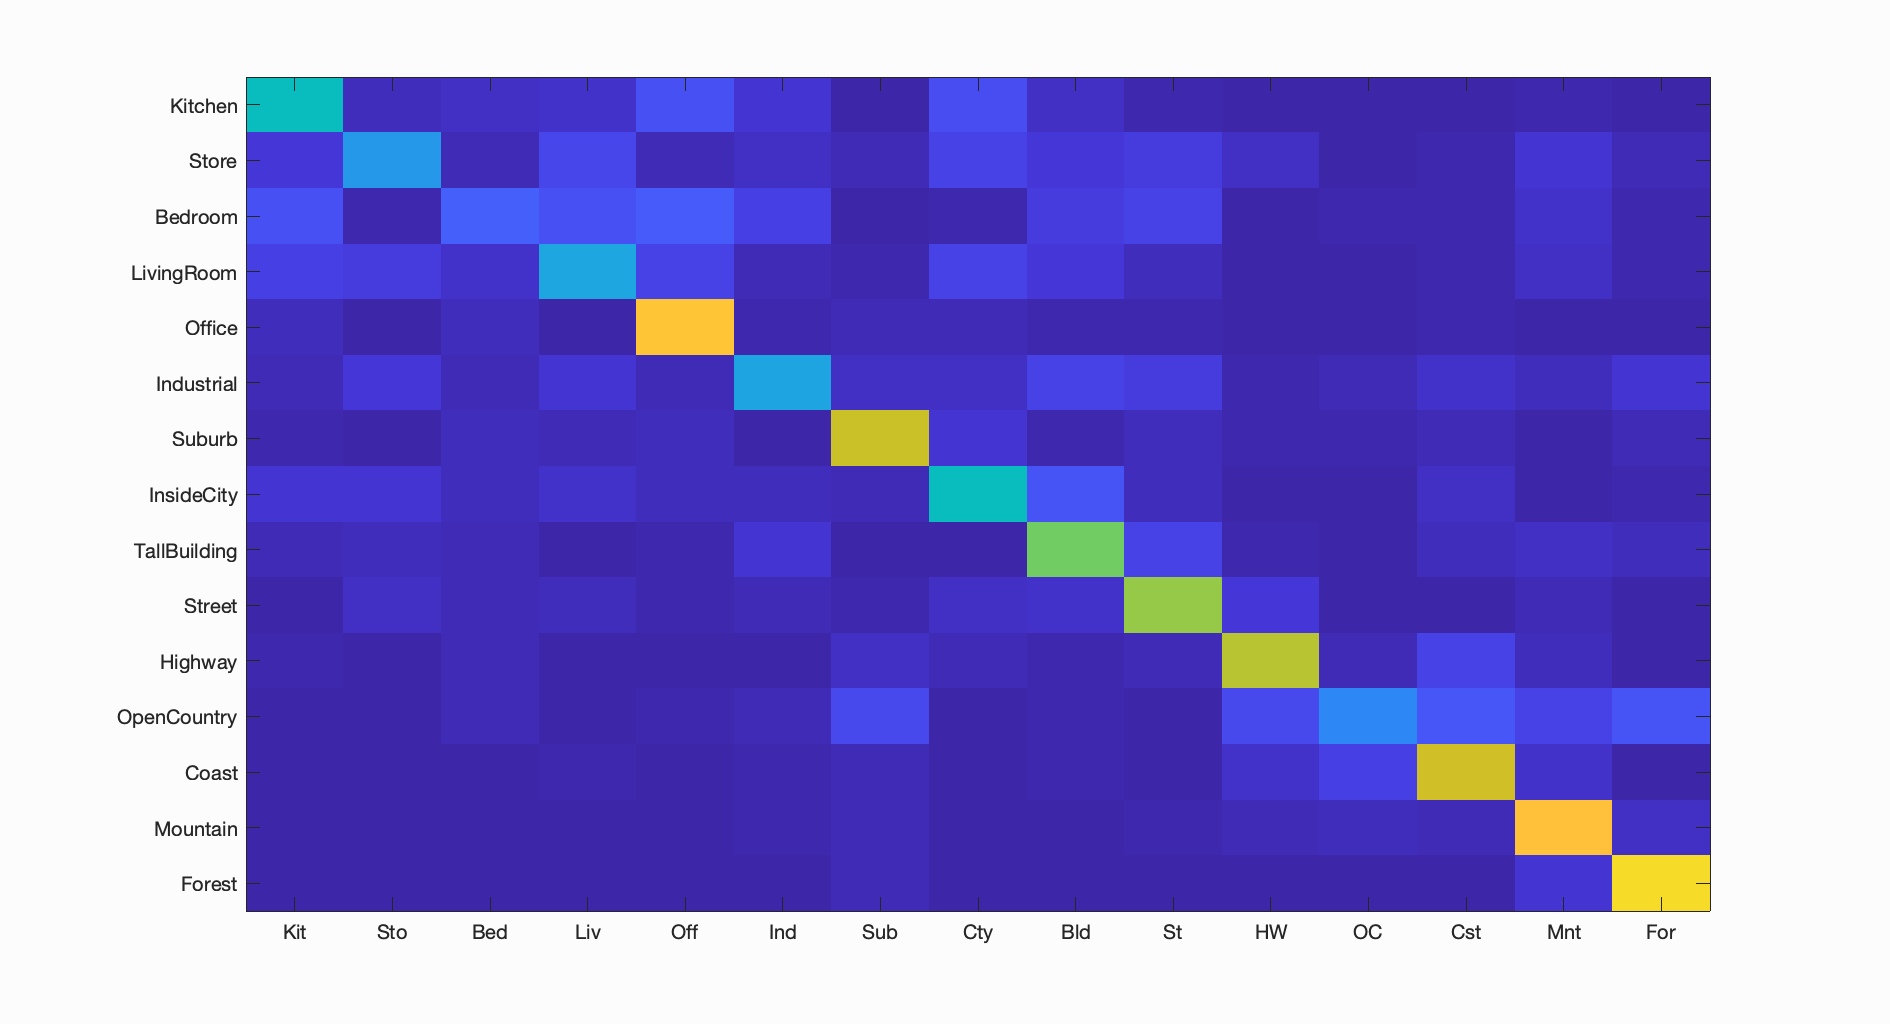
\includegraphics[width=8cm]{confusion_matrix.png}
    \caption{Confusion Matrix from Bags of Words + SVM}
\end{figure}

\begin{figure}[h!]
    \centering
    \captionsetup{justification=centering}
    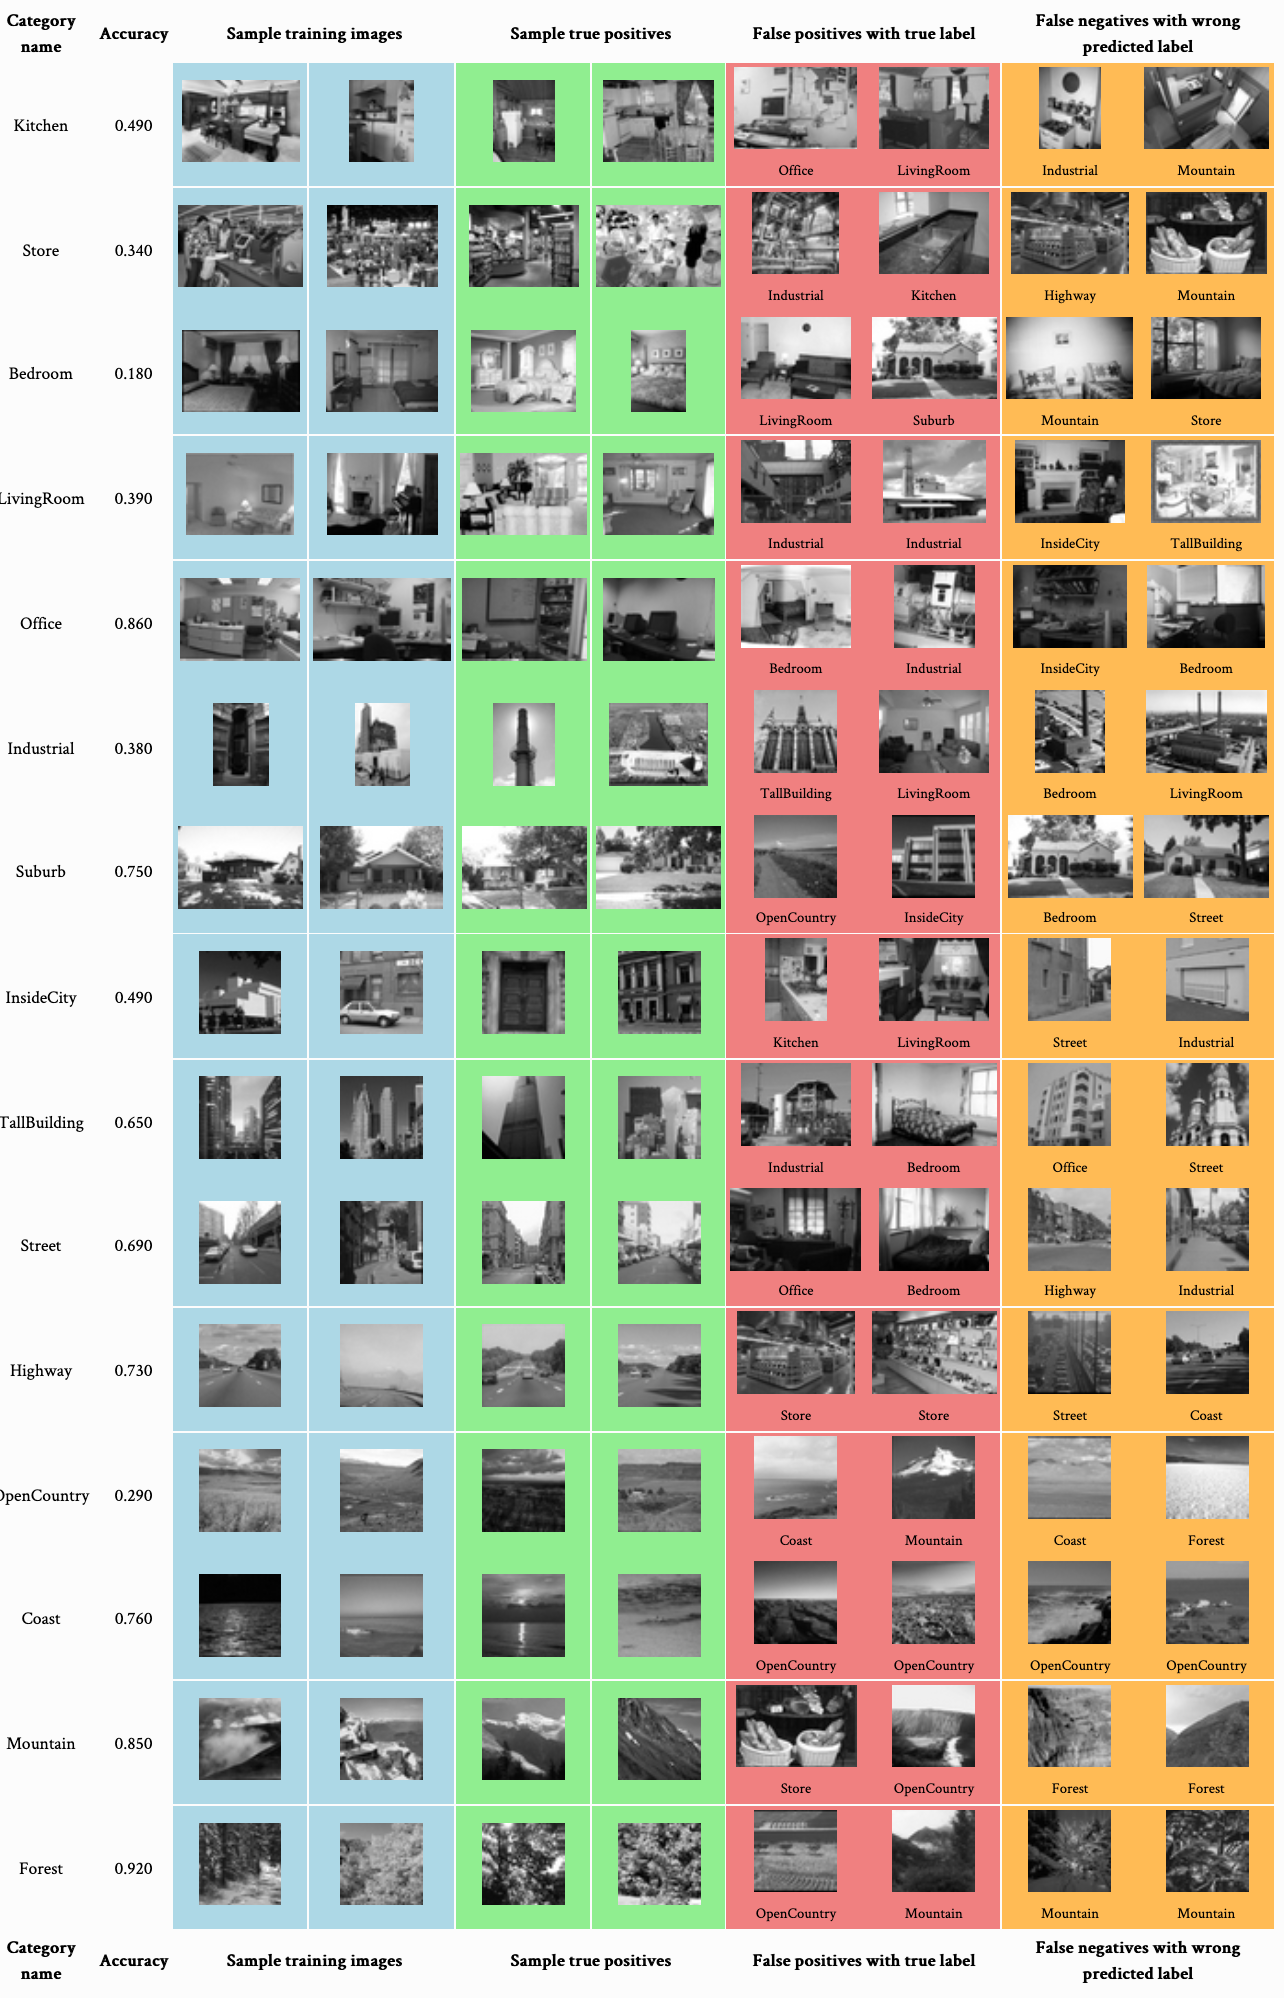
\includegraphics[width=8cm]{table.png}
    \caption{Table of classifier results from Bags of Words + SVM}
\end{figure}
\end{document}
